\chapter{Results}
\label{ch:Results}

The following results demonstrate the versatility of our method. Our implementation relied on the
Ipopt non-linear optimization package \cite{Wachter:2006} to solve the constrained optimization
problem proposed in equation~\eqref{eq:constrained-min}.  We use a tetrahedral mesh discretization for
all our simulations.

\subsection{Two Tetrahedrons}

As the most simple proof of concept example for the volume constraint, we design a mesh with two
tetrahedrons with equal volume joined together by a face as shown in Figure~\ref{fig:twotets}. We
then compress one of the tetrahedrons with a Dirichlet boundary condition to a plane, to see the
effects of the volume constraint. The energy model used is Neo-Hookean with $\nu = 0.495$. 

As expected, the example without the global volume constraint loses around $50\%$ of the volume,
since the deformation of the compressed tetrahedron does not affect its neighbor.
When a volume constraint is applied, the unconstrained tetrahedron inflates to twice the original
size, keeping the total volume constant. 


\subsection{Twist}

\begin{figure}[ht]
	\centering
	\begin{tabular}{l|cccc}
		& UNH & Penalty, $\beta = 9$ & CNH & CNH + Epi \\
		\midrule
		$\frac{\pi}{2}$ &
		\begin{subfigure}{.2\linewidth}
			\centering
			\adjustbox{trim={.2\width} {.00\height} {.2\width} {.00\height},clip}%
			{\includegraphics[width=2.0\textwidth]{images/twist/pr100-1.png}}
			%\caption*{(a1)}
			\label{sfig:twist-035-1}
		\end{subfigure} &
		\begin{subfigure}{.2\linewidth}
			\centering
			\adjustbox{trim={.2\width} {.00\height} {.2\width} {.00\height},clip}%
			{\includegraphics[width=2.0\textwidth]{images/twist/vp100-1.png}}
			%\caption*{(b1)}
			\label{sfig:twist-035-vc-1}
		\end{subfigure} &
		\begin{subfigure}{.2\linewidth}
			\centering
			\adjustbox{trim={.2\width} {.00\height} {.2\width} {.00\height},clip}%
			{\includegraphics[width=2.0\textwidth]{images/twist/vc100-1.png}}
			%\caption*{(c1)}
			\label{sfig:twist-035-vcip-1}
		\end{subfigure} &
		\begin{subfigure}{.2\linewidth}
			\centering
			\adjustbox{trim={.2\width} {.00\height} {.2\width} {.00\height},clip}%
			{\includegraphics[width=2.0\textwidth]{images/twist/vc100_epi20-1.png}}
			%\caption*{(d1)}
			\label{sfig:twist-035-vc-1-epi}
		\end{subfigure} \\
		$\pi$ &
		\begin{subfigure}{.2\linewidth}
			\centering
			\adjustbox{trim={.2\width} {.00\height} {.2\width} {.00\height},clip}%
			{\includegraphics[width=2.0\textwidth]{images/twist/pr100-2.png}}
			%\caption*{(a2)}
			\label{sfig:twist-035-2}
		\end{subfigure} &
		\begin{subfigure}{.2\linewidth}
			\centering
			\adjustbox{trim={.2\width} {.00\height} {.2\width} {.00\height},clip}%
			{\includegraphics[width=2.0\textwidth]{images/twist/vp100-2.png}}
			%\caption*{(b2)}
			\label{sfig:twist-035-vc-2}
		\end{subfigure} &
		\begin{subfigure}{.2\linewidth}
			\centering
			\adjustbox{trim={.2\width} {.00\height} {.2\width} {.00\height},clip}%
			{\includegraphics[width=2.0\textwidth]{images/twist/vc100-2.png}}
			%\caption*{(c2)}
			\label{sfig:twist-035-vcip-2}
		\end{subfigure} &
		\begin{subfigure}{.2\linewidth}
			\centering
			\adjustbox{trim={.2\width} {.00\height} {.2\width} {.00\height},clip}%
			{\includegraphics[width=2.0\textwidth]{images/twist/vc100_epi20-2.png}}
			%\caption*{(d2)}
			\label{sfig:twist-035-vc-2-epi}
		\end{subfigure} \\
		$\frac{\pi}{3}$ &
		\begin{subfigure}{.2\linewidth}
			\centering
			\adjustbox{trim={.2\width} {.00\height} {.2\width} {.00\height},clip}%
			{\includegraphics[width=2.0\textwidth]{images/twist/pr100-3.png}}
			\caption*{(a)}
			\label{sfig:twist-035-3}
		\end{subfigure} &
		\begin{subfigure}{.2\linewidth}
			\centering
			\adjustbox{trim={.2\width} {.00\height} {.2\width} {.00\height},clip}%
			{\includegraphics[width=2.0\textwidth]{images/twist/vp100-3.png}}
			\caption*{(b)}
			\label{sfig:twist-035-vc-3}
		\end{subfigure} &
		\begin{subfigure}{.2\linewidth}
			\centering
			\adjustbox{trim={.2\width} {.00\height} {.2\width} {.00\height},clip}%
			{\includegraphics[width=2.0\textwidth]{images/twist/vc100-3.png}}
			\caption*{(c)}
			\label{sfig:twist-035-vcip-3}
		\end{subfigure} &
		\begin{subfigure}{.2\linewidth}
			\centering
			\adjustbox{trim={.2\width} {.00\height} {.2\width} {.00\height},clip}%
			{\includegraphics[width=2.0\textwidth]{images/twist/vc100_epi20-3.png}}
			\caption*{(d)}
			\label{sfig:twist-035-vc-3-epi}
		\end{subfigure} \\
	\end{tabular}
	\caption{\textbf{Cube Twist Simulation}: The top face of a cube with $15^3$ vertices is
		rotated by $\frac{\pi}{2}$ (top row), by $\pi$ (middle row), and by $\frac{3 \pi}{2}$. (a)
		is the basic Stable Neo-Hookean simulation with $\lambda = 100$, (b) is a UNH simulation
		using our penalty with $\lambda = 100, \beta = 9$, (c) is a constrained simulation where a
		global zone is used in addition to the penalty, and (d) is a simulation where epidermis of
		$\lambda = 15, \gamma = 1$ is added. We notice that where the Stable Neo-Hookean simulation
		fails, while the additional non-linearity introduced by the compression penalty successfully
		resolves inversions. Adding the volume constraint allows a completely incompressible
		simulation, and applying the epidermis model results in an organic looking deformation.}
	\label{fig:twist}
\end{figure} 

We adopt the classic twisting cube test to verify the robustness of our method. We fix the two sides
of a $15^3$ cube, and twist one of the fixed sides by $\frac{\pi}{2}$ three times. With $\mu = 4.0,
\lambda = 100.0$ the basic Stable Neo-Hookean simulation loses 6.45\% of the volume in the
initial two rotations, then collapses from severe inversions. Adding additional non-linearity to the volumetric energy density function of $\beta = 9.0$, we are able to completely remove the inversions and achieve a robust simulation to the end, while the volume error remains almost the same. By imposing a volume constraint on the global zone, the volume is preserved completely. Finally, adding an epidermis model of $\lambda = 15.0, \gamma = 1.0$ results in a more organic surface deformation.

\subsection{Standing Cube}

\begin{figure*}
	\centering
	\begin{subfigure}{.32\linewidth}
		\centering
		\adjustbox{trim={.15\width} {.00\height} {.15\width} {.00\height},clip}%
		{\includegraphics[width=1.0\textwidth]{images/suspended_cube/pr0495.png}}
		\caption*{(a) UNH, $\nu = 0.495$}
		\label{sfig:suspended-cube-pr-0495}
	\end{subfigure}%
	\begin{subfigure}{.32\linewidth}
		\centering
		\adjustbox{trim={.15\width} {.00\height} {.15\width} {.00\height},clip}%
		{\includegraphics[width=1.0\textwidth]{images/suspended_cube/onering.png}}
		\caption*{(b) One-ring}
		\label{sfig:suspended-cube-onering}
	\end{subfigure}%
	\begin{subfigure}{.32\linewidth}
		\centering
		\adjustbox{trim={.15\width} {.00\height} {.15\width} {.00\height},clip}%
		{\includegraphics[width=1.0\textwidth]{images/suspended_cube/vc100.png}}
		\caption*{(c) CNH, $\lambda = 100, \beta = 1$}
		\label{sfig:suspended-cube-vc-100}
	\end{subfigure}%
	\caption{\textbf{Suspended Cube}: A cube with $12^3$ vertices is suspended under gravity with the bottom surface fixed with Dirichlet boundary conditions, visualized with the per-tet pressure distribution in the inner body. (a) shows the per-tet Poisson's ratio approach with $\nu = 0.495$, where the effects of volumetric locking results in highly irregular pressure distribution. (b) is the result where a one-ring volume constraint is used, where a checkerboard pattern appears in the pressure distribution due to a lack of stability. Finally, (c) is our method with $\lambda = 100, \beta = 1$, where the pressure distribution is regular and realistic. }
	\label{fig:suspended-cubes}
\end{figure*}

Following a classic volumetric locking example, we test our methods with a standing cube simulation. A Neo-Hookean cube with shear modulus $\mu = 10.0$ is suspended under gravity with the bottom surface fixed with Dirichlet boundary conditions, results shown in Figure~\ref{fig:suspended-cubes}. This example demonstrates the effects of external force on the pressure distribution on the body surface and interior with regards to different approaches of simulating incompressibility. Irregular pressure distribution may not visually affect the results much, but when simulating frictional contact or fracture, they might result in unrealistic solutions. The high Poisson's ratio ($\nu = 0.495$) approach results in obvious irregularities in the pressure distribution, a manifestation of volumetric locking. The per-tet hydrostatic pressures in this case are computed as the the volumetric components of the stress tensors, that is, the negative divergence of the Cauchy stress. The high bulk modulus per each element causes pressure computation from displacement variables to be unreliable. The one-ring volume constraint approach \cite{Irving:2007}, which is equivalent to the Average Nodal Pressure element \cite{bonet:1998}, shows a more regular pressure distribution, but also shows checkerboard patterns. In this case, the pressures are the Lagrange multipliers for the volume constraints, scaled to be in the same units as the volumetric stress then mapped back to the cells. The checkerboard pattern is an artifact of the instability of the one-ring constraint approach, where the averaging of the pressure variables on the nodes allows solutions with such checkerboarding to occur. With our method with one global zone and a penalty of $\lambda = 100, \beta = 1$, we compute the per-tet pressure as a sum of the average zonal pressure (the Lagrange multiplier of the zonal volume constraint) and the fine-scale pressures computed from the volumetric stress component from the penalty. Then since the bulk modulus is much smaller, as opposed to $(\nu = 0.495) \equiv (\lambda = 400)$ in the Poisson's ratio approach, volumetric locking does not happen from the penalty, and therefore the volumetric stress components are more regular. Since the volume preserving zone is global and since the average pressure is constant throughout the zone, checkerboard pattern in the Lagrange multipliers is not an issue. 

\subsection{Stability Test}

\begin{figure}
	\centering   	
	\begin{overpic}[width=1.0\columnwidth]{images/stability.pdf}
		\put(30,30){\includegraphics[width=0.3\columnwidth]{images/rep.png}}  
		\put(49.5,14){
			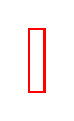
\begin{tikzpicture}
			\draw[thick,draw=red] (0,0) rectangle ++(0.2,0.8);
			\end{tikzpicture}	
		}
	\end{overpic} \hfill
	\begin{overpic}[width=0.5\columnwidth]{images/energy_plot_zoom.pdf}
		\put(0,-0.2){
			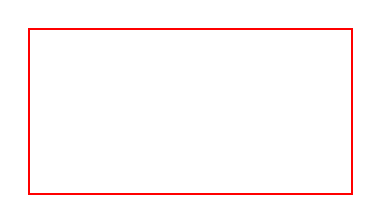
\begin{tikzpicture}
			\draw[thick,draw=red] (0,0) rectangle ++(4.1,2.1);
			\end{tikzpicture}	
		}
	\end{overpic}
	\caption{Energy plot from the simulation of a soft $16^3$ cell cube subjected to gravity, with a moderately large timestep of 8ms. We compare three different algorithms for simulating incompressibility, where the blue curve is the energy plot for the one-ring pressure algorithm of \cite{Irving:2007}, the red is a na\"ive global volume rescaling algorithm, and yellow is ours. \cite{Irving:2007} (blue) shows severe instability even with an aggressive clamping of the volume recovery. Note how due to the extreme oscillations in potential energy, the energy plot for the method appears as a thick line in the top plot. The bottom plot shows a magnified plot to demonstrate how the energy behaves in small timeframe. The volume rescaling algorithm (red) gains and loses energy arbitrarily due to a unrealistic simulation of the volumetric stress, which can be seen from the irregularities in the plot. Our method (yellow) displays a realistic and stable energy behavior, and converges to a stable configuration. \label{fig:stability}}
\end{figure}

\new{
	We test the stability of our method in dyanamic simulations compared to \cite{Irving:2007} and a na\"ive volume rescaling method. We simulate a cube consisting of $16^3$ cells with $\mu = 100.0$ is subjected under gravity. We tested the simulation with a timestep of 8ms for a total of 1000 frames.
	We found that the volume projection in the Irving algorithm can be unstable when used with large timesteps and a clamping of volume preservation forces must be applied to make it stable. However, we found that the clamping threshold to make this specific example not blow up was quite low, resulting in a volume error of ~2.4\% at worst. Even with such aggressive clamping, we noticed visible oscillations on the top surface of the cube.
	We tested a simple volume rescaling algorithm where the mesh was readjusted based on its center of mass such that the global volume is conserved. We found that this method is highly unstable virtually impossible with Semi-Implicit Euler integration without increasing Poisson Ratio to higher than 0.495, where then locking occurs instead. With full Backwards Euler, we could get the simulation to not blow up, but it still required a quite high Poisson Ratio of 0.48. However, a unrealistically exaggerated oscillation of the entire mesh was present even until the final frames.
	Compared to the other methods, we found our method to be very stable, and the runtimes were comparable (around 2\% faster) to Irving's, which is a semi-implicit method where ours is fully implicit. With our method, this simulation can even be stably run at much higher timesteps, i.e. 33ms. 
}

\new{
	The plot of the potential energy for this simulation can be seen Figure~\ref{fig:stability}. Note the extreme oscillations present in the potential energy plot for the one-ring nodal pressure algorithm \cite{Irving:2007} and the unrealistic irregularities in the plot for the volume rescaling algorithm.
	For a visual comparison of the instabilities of the other two methods compared to ours, please refer to our accompanied video.
}
\subsection{Cube Stretch}
We demonstrate the inversion robustness and performance of our method with a stretching cube example, where a regularly discretized cube of dimensions $20 \times 20 \times 20$ is stretched to 8 times its original length. In all cases, $\mu = 1.0$, and the relative tolerance for Ipopt was $1e-6$. Using an unconstrained Stable Neo-Hookean energy with $\lambda = 10.0$ (or $\nu \approx 0.4545$), the runtime was 2.803 seconds per frame. However, there were severe tet inversions in the final frames and the volume error was ~14.83\%. With $\lambda = 100.0$ (or $\nu = 0.495$) the tet inversions were removed and the volume error was reduced to ~5.05\%, but the runtime per frame increased to 9.905 seconds per frame.

With the volume constraint added and using a penalty of $\lambda = 25, \beta = 0$ (equivalent to Stable Neo-Hookean), the runtime per frame was 7.892 seconds. The inversions were completely removed and the volume was accurately preserved. By increasing $\beta$ to 1, the performance improved by ~8.38\% to 7.282 seconds per frame. When epidermis ($\lambda_e = 10.0, \gamma = 1.0$) was added, the performance improved to 6.251 seconds per frame, while producing a more organic looking result.

\begin{figure}
	\centering
	\begin{subfigure}{1.0\linewidth}
		\centering
		\adjustbox{trim={.05\width} {.3\height} {.05\width} {.3\height},clip}%
		{\includegraphics[width=1.0\textwidth]{images/cube_stretch/pr04545.jpg}}
		\caption*{(a) UNH, $\lambda = 10$}
		\label{sfig:stretch-snh10}
	\end{subfigure}\par\medskip
	\begin{subfigure}{1.0\linewidth}
		\centering
		\adjustbox{trim={.05\width} {.3\height} {.05\width} {.3\height},clip}%
		{\includegraphics[width=1.0\textwidth]{images/cube_stretch/pr0495.jpg}}
		\caption*{(b) UNH, $\lambda = 100$}
		\label{sfig:stretch-snh100}
	\end{subfigure}\par\medskip
	\begin{subfigure}{1.0\linewidth}
		\centering
		\adjustbox{trim={.05\width} {.3\height} {.05\width} {.3\height},clip}%
		{\includegraphics[width=1.0\textwidth]{images/cube_stretch/vc25-1.jpg}}
		\caption*{(c) CNH, $\lambda = 25$}
		\label{sfig:stretch-vc}
	\end{subfigure}\par\medskip
	\begin{subfigure}{1.0\linewidth}
		\centering
		\adjustbox{trim={.05\width} {.3\height} {.05\width} {.3\height},clip}%
		{\includegraphics[width=1.0\textwidth]{images/cube_stretch/vc25-1_epi10-1.jpg}}
		\caption*{(d) CNH + Epidermis}
		\label{sfig:stretch-vcepi}
	\end{subfigure}%
	\caption{\textbf{Cube Stretch}: A cube is stretched with two moving Dirichlet boundaries on the sides and stretched to eight times of its original length. (a) Using the unconstrained Stable Neo-Hookean with $\nu \approx 0.4545$, the volume error was ~14.83\% and tets became inverted around the cube corners (purple tets). (b) With $\nu = 0.495$, inverted tets were removed and the volume error is reduced to ~5.05\%. (c) When volume constraint ($\lambda = 25, \beta = 1$) is introduced, the volume is completely preserved and we are able to achieve a visually similar result with 26.54\% faster runtime per frame. (d) With the epidermis ($\lambda_e = 10, \gamma = 1$) the deformed surface is regularized and the resulting deformation looks more organic. }
	\label{fig:cube-stretch}
\end{figure}

\subsection{Skin Puck Simulation}

\begin{figure*}
	\centering
	\begin{subfigure}{.24\linewidth}
		\centering
		\includegraphics[width=1.0\textwidth]{images/puck/pr0495_25.png}
		\includegraphics[width=1.0\textwidth]{images/puck/pr0495_50.png}
		\caption*{(a) UNH, $\nu = 0.495$}
		\label{sfig:puck-pr0495}
	\end{subfigure}
	\begin{subfigure}{.24\linewidth}
		\centering
		\includegraphics[width=1.0\textwidth]{images/puck/pr04545_25.png}
		\includegraphics[width=1.0\textwidth]{images/puck/pr04545_50.png}
		\caption*{(b) UNH, $\nu = 0.4545$}
		\label{sfig:puck-pr04545}
	\end{subfigure}%
	\begin{subfigure}{.24\linewidth}
		\centering
		\includegraphics[width=1.0\textwidth]{images/puck/vc60-15_25.png}
		\includegraphics[width=1.0\textwidth]{images/puck/vc60-15_50.png}
		\caption*{(c) CNH}
		\label{sfig:puck-vc}
	\end{subfigure}%
	\begin{subfigure}{.24\linewidth}
		\centering
		\includegraphics[width=1.0\textwidth]{images/puck/vc60-15_epi40_25.png}
		\includegraphics[width=1.0\textwidth]{images/puck/vc60-15_epi40_50.png}
		\caption*{(d) CNH + Epidermis}
		\label{sfig:puck-vc-epi}
	\end{subfigure}%
	\caption{\textbf{Skin Puck Simulations}: A puck, fixed on the bottom, is displaced with a Dirichlet boundary condition on a circular region in the top surface. (a) is the clipped result of the simulation without volume constraint and per-tet Poisson's ratio $\nu = 0.495$, at indentations of $25\%$ and $50\%$ of the puck height. These base results show visible volume loss of $0.6\%$ and $1.8\%$ and artificial stiffness from locking, resulting in no visible bulging at the cylinder top. Also, the pressure distribution visualized by the color scheme shows severe irregularities. (b) is the simulation with per-tet bulk modulus $\nu = 0.4545$, which loses $2.1\%$ and $5.1\%$ of the total volume respectively, and inverted elements (yellow) occur around the indentation boundary. (c) shows the result with volume constraint and $\lambda = 40$ (equivalent to $\nu = 0.4545$) and $\beta = 15$, showing a realistic bulging due to successful volume preservation, and the inversions are removed. The pressure distribution is also regularized and natural. (d) shows the result where an epidermis of $\lambda = 40$ was added, where the surface demonstrates a more organic deformation due to surface volume preservation. }
	\label{fig:pucks}
\end{figure*} 

One good natural example of an incompressible material is the human tissue, so to test the effects of our method, we test on the ``skin puck'' model from \cite{Pai:2018}, where the vertices on the bottom are fixed with Dirichlet boundary conditions. We use a 22K tetrahedron simulation mesh for the puck.  To produce substantial compression, we animate a set of vertices on the top of the puck with a Dirichlet boundary condition moving these vertices down by a fixed amount per time step. We performed a quasi-static simulation where at each step, the animated surface is indented by 1\% of the height. We test the displacement until 50\% of the total height of the puck, which produces extreme compression.

Without the volume constraint, a low Poisson's Ratio $\nu \in [0.0, 0.45]$ will result in little noticeable bulging at the top surface due to volume loss, and a higher $\nu$ will result in unnaturally stiff visual results and irregular pressure distribution due to volumetric locking. Also, even at $\nu = 0.495$, there was a $1.8\%$ volume loss at an indentation of 50\% of the puck height.

Adding the volume constraint allows a completely incompressible simulation with realistic pressure solutions for this example, without being a heavy burden on the performance in most cases. At $50\%$ indentation, the amount of volume loss can be made arbitrarily low\footnote{Up to machine precision.} with the global volume constraint using any type of energy model and parameters. In contrast, a standard simulation without the constraint produces approximately 22\% volume loss with $\nu = 0.4$, 5.1\% loss with $\nu = 0.45$, and 1.8\% loss with $\nu = 0.495$. However, without any local volumetric penalty the simulation converges to an infeasible state with many inverted tets around the border of the Dirichet boundaries.

Adding our per-tet penalty term of $\lambda = 60$ (equivalent to $\nu = 0.4681$) allows the simulation to be completely free of inverted tets. Although even with $\beta = 0$ the solution does not converge to an infeasible state, the lack of a sufficient resistance to volumetric deformation causes numerical instability and results in a very slow convergence of the nonlinear optimizer during the timesteps with more extreme deformations (after the 25\% indentation). By using $\beta = 15$ we were able to achieve better numerical stability, resulting in a 14.84\% faster runtime on total, and 21.17\% faster runtime when only considering the frames after the 25\% indentation where the moving Dirichlet boundary starts to invert elements. Finally, with an epidermis model of $\lambda_e = 40, \beta_e = 1$ added, we are able to generate a more regular surface deformation and achieve an visually organic deformation overall. 

\subsection{Ball Drop}

\begin{figure*}[htp!]
	\centering
	\begin{subfigure}{.03\linewidth}
		\rotatebox[origin=c]{90}{\footnotesize{\quad(a) UNH, $\nu=0.45$}}
	\end{subfigure}%
	\begin{subfigure}{.16\linewidth}
		\centering
		\adjustbox{trim={.25\width} {.0\height} {.25\width} {.4\height},clip}%
		{\includegraphics[width=2.0\textwidth]{images/soft_ball/045/0200.jpg}}
		%\caption*{(a1)}
		\label{sfig:ball-045-1}
	\end{subfigure}%
	\begin{subfigure}{.16\linewidth}
		\centering
		\adjustbox{trim={.25\width} {.0\height} {.25\width} {.4\height},clip}%
		{\includegraphics[width=2.0\textwidth]{images/soft_ball/045/0250.jpg}}
		%\caption*{(a2)}
		\label{sfig:ball-045-2}
	\end{subfigure}%
	\begin{subfigure}{.16\linewidth}
		\centering
		\adjustbox{trim={.25\width} {.0\height} {.25\width} {.4\height},clip}%
		{\includegraphics[width=2.0\textwidth]{images/soft_ball/045/0300.jpg}}
		%\caption*{(a3)}
		\label{sfig:ball-045-3}
	\end{subfigure}%
	\begin{subfigure}{.16\linewidth}
		\centering
		\adjustbox{trim={.25\width} {.0\height} {.25\width} {.4\height},clip}%
		{\includegraphics[width=2.0\textwidth]{images/soft_ball/045/0350.jpg}}
		%\caption*{(a4)}
		\label{sfig:ball-045-4}
	\end{subfigure}%
	\begin{subfigure}{.16\linewidth}
		\centering
		\adjustbox{trim={.25\width} {.0\height} {.25\width} {.4\height},clip}%
		{\includegraphics[width=2.0\textwidth]{images/soft_ball/045/0400.jpg}}
		%\caption*{(a5)}
		\label{sfig:ball-045-5}
	\end{subfigure}%
	\begin{subfigure}{.16\linewidth}
		\centering
		\adjustbox{trim={.25\width} {.0\height} {.25\width} {.4\height},clip}%
		{\includegraphics[width=2.0\textwidth]{images/soft_ball/045/0450.jpg}}
		%\caption*{(a6)}
		\label{sfig:ball-045-6}
	\end{subfigure}\hfill
	\begin{subfigure}{.03\linewidth}
		\rotatebox[origin=c]{90}{\footnotesize{\quad(b) UNH, $\nu=0.495$}}
	\end{subfigure}%
	\begin{subfigure}{.16\linewidth}
		\centering
		\adjustbox{trim={.25\width} {.0\height} {.25\width} {.4\height},clip}%
		{\includegraphics[width=2.0\textwidth]{images/soft_ball/0495/0200.jpg}}
		%\caption*{(a1)}
		\label{sfig:ball-0495-1}
	\end{subfigure}%
	\begin{subfigure}{.16\linewidth}
		\centering
		\adjustbox{trim={.25\width} {.0\height} {.25\width} {.4\height},clip}%
		{\includegraphics[width=2.0\textwidth]{images/soft_ball/0495/0250.jpg}}
		%\caption*{(a2)}
		\label{sfig:ball-0495-2}
	\end{subfigure}%
	\begin{subfigure}{.16\linewidth}
		\centering
		\adjustbox{trim={.25\width} {.0\height} {.25\width} {.4\height},clip}%
		{\includegraphics[width=2.0\textwidth]{images/soft_ball/0495/0300.jpg}}
		%\caption*{(a3)}
		\label{sfig:ball-0495-3}
	\end{subfigure}%
	\begin{subfigure}{.16\linewidth}
		\centering
		\adjustbox{trim={.25\width} {.0\height} {.25\width} {.4\height},clip}%
		{\includegraphics[width=2.0\textwidth]{images/soft_ball/0495/0350.jpg}}
		%\caption*{(a4)}
		\label{sfig:ball-0495-4}
	\end{subfigure}%
	\begin{subfigure}{.16\linewidth}
		\centering
		\adjustbox{trim={.25\width} {.0\height} {.25\width} {.4\height},clip}%
		{\includegraphics[width=2.0\textwidth]{images/soft_ball/0495/0400.jpg}}
		%\caption*{(a5)}
		\label{sfig:ball-0495-5}
	\end{subfigure}%
	\begin{subfigure}{.16\linewidth}
		\centering
		\adjustbox{trim={.25\width} {.0\height} {.25\width} {.4\height},clip}%
		{\includegraphics[width=2.0\textwidth]{images/soft_ball/0495/0450.jpg}}
		%\caption*{(a6)}
		\label{sfig:ball-0495-6}
	\end{subfigure}\hfill
	\begin{subfigure}{.03\linewidth}
		\rotatebox[origin=c]{90}{\footnotesize{\quad(c) Ours}}
	\end{subfigure}%
	\begin{subfigure}{.16\linewidth}
		\centering
		\adjustbox{trim={.25\width} {.0\height} {.25\width} {.4\height},clip}%
		{\includegraphics[width=2.0\textwidth]{images/soft_ball/vp/0200.jpg}}
		%\caption*{(a1)}
		\label{sfig:ball-vc-1}
	\end{subfigure}%
	\begin{subfigure}{.16\linewidth}
		\centering
		\adjustbox{trim={.25\width} {.0\height} {.25\width} {.4\height},clip}%
		{\includegraphics[width=2.0\textwidth]{images/soft_ball/vp/0250.jpg}}
		%\caption*{(a2)}
		\label{sfig:ball-vc-2}
	\end{subfigure}%
	\begin{subfigure}{.16\linewidth}
		\centering
		\adjustbox{trim={.25\width} {.0\height} {.25\width} {.4\height},clip}%
		{\includegraphics[width=2.0\textwidth]{images/soft_ball/vp/0300.jpg}}
		%\caption*{(a3)}
		\label{sfig:ball-vc-3}
	\end{subfigure}%
	\begin{subfigure}{.16\linewidth}
		\centering
		\adjustbox{trim={.25\width} {.0\height} {.25\width} {.4\height},clip}%
		{\includegraphics[width=2.0\textwidth]{images/soft_ball/vp/0350.jpg}}
		%\caption*{(a4)}
		\label{sfig:ball-vc-4}
	\end{subfigure}%
	\begin{subfigure}{.16\linewidth}
		\centering
		\adjustbox{trim={.25\width} {.0\height} {.25\width} {.4\height},clip}%
		{\includegraphics[width=2.0\textwidth]{images/soft_ball/vp/0400.jpg}}
		%\caption*{(a5)}
		\label{sfig:ball-vc-5}
	\end{subfigure}%
	\begin{subfigure}{.16\linewidth}
		\centering
		\adjustbox{trim={.25\width} {.0\height} {.25\width} {.4\height},clip}%
		{\includegraphics[width=2.0\textwidth]{images/soft_ball/vp/0450.jpg}}
		%\caption*{(a6)}
		\label{sfig:ball-vc-6}
	\end{subfigure}\hfill
	\begin{subfigure}{.03\linewidth}
		\rotatebox[origin=c]{90}{\footnotesize{\quad Frame}}
	\end{subfigure}%
	\begin{subfigure}{.16\linewidth}
		\centering
		200
	\end{subfigure}%
	\begin{subfigure}{.16\linewidth}
		\centering
		250
	\end{subfigure}%
	\begin{subfigure}{.16\linewidth}
		\centering
		300
	\end{subfigure}%
	\begin{subfigure}{.16\linewidth}
		\centering
		350
	\end{subfigure}%
	\begin{subfigure}{.16\linewidth}
		\centering
		400
	\end{subfigure}%
	\begin{subfigure}{.16\linewidth}
		\centering
		450
	\end{subfigure}%
	\caption{\textbf{Ball Drop}: An elastic sphere consisting of 64K tets is dropped to the ground. (a) shows the result with the standard UNH model with per-tet Poisson's ratio $\nu = 0.45$, where the ball loses more than half its volume in the second column. (b) is the UNH result with $\nu = 0.495$, where the volumetric locking makes the ball appear unnaturally stiff. Notice how the ball always retains its spherical shape and just get flattened and stretched in the vertical direction. (c) is the result using our CNH model with global volume constraint and compression penalty with $\lambda$ equivalent to $\nu = 0.45$. Note that the volume of the sphere is preserved, producing a nice ``squash-and-stretch'' effect, and the artificial stiffness is removed.} \label{fig:fine-ball}
\end{figure*}

\new{
	We test a simple dynamic result of a soft ball consisting of 64K tets dropped under gravity and dropped to the ground in Figure~\ref{fig:fine-ball}. We used a timestep of 1ms and $\mu = 16.0$ KPa. Using a per-tet Poisson's ratio $\nu = 0.495$ results in the sphere behaving much stiffer than what the material parameters would suggest, while still losing up to 12.7\% of its volume. When using a per-tet Poisson's ratio of $\nu = 0.45$, the ball retains its appearance of soft elastic deformation, but loses up to 51\% of its original volume. Using our method, we are able to simulate the soft elastic deformations while preserving the volume down to solver accuracy, while being 5.7\% faster than the high Poisson's ratio case and only 3.7\% slower than the $\nu=0.45$ case. 
}

\begin{figure*}[htp!]
	\centering
	\begin{subfigure}{.03\linewidth}
		\rotatebox[origin=c]{90}{\footnotesize{\quad(a) UNH, $\nu=0.45$}}
	\end{subfigure}%
	\begin{subfigure}{.16\linewidth}
		\centering
		\adjustbox{trim={.25\width} {.0\height} {.25\width} {.4\height},clip}%
		{\includegraphics[width=2.0\textwidth]{images/coarse_ball/045/0200.jpg}}
		%\caption*{(a1)}
		\label{sfig:ball-045-1}
	\end{subfigure}%
	\begin{subfigure}{.16\linewidth}
		\centering
		\adjustbox{trim={.25\width} {.0\height} {.25\width} {.4\height},clip}%
		{\includegraphics[width=2.0\textwidth]{images/coarse_ball/045/0250.jpg}}
		%\caption*{(a2)}
		\label{sfig:ball-045-2}
	\end{subfigure}%
	\begin{subfigure}{.16\linewidth}
		\centering
		\adjustbox{trim={.25\width} {.0\height} {.25\width} {.4\height},clip}%
		{\includegraphics[width=2.0\textwidth]{images/coarse_ball/045/0300.jpg}}
		%\caption*{(a3)}
		\label{sfig:ball-045-3}
	\end{subfigure}%
	\begin{subfigure}{.16\linewidth}
		\centering
		\adjustbox{trim={.25\width} {.0\height} {.25\width} {.4\height},clip}%
		{\includegraphics[width=2.0\textwidth]{images/coarse_ball/045/0350.jpg}}
		%\caption*{(a4)}
		\label{sfig:ball-045-4}
	\end{subfigure}%
	\begin{subfigure}{.16\linewidth}
		\centering
		\adjustbox{trim={.25\width} {.0\height} {.25\width} {.4\height},clip}%
		{\includegraphics[width=2.0\textwidth]{images/coarse_ball/045/0400.jpg}}
		%\caption*{(a5)}
		\label{sfig:ball-045-5}
	\end{subfigure}%
	\begin{subfigure}{.16\linewidth}
		\centering
		\adjustbox{trim={.25\width} {.0\height} {.25\width} {.4\height},clip}%
		{\includegraphics[width=2.0\textwidth]{images/coarse_ball/045/0450.jpg}}
		%\caption*{(a6)}
		\label{sfig:ball-045-6}
	\end{subfigure}\hfill
	\begin{subfigure}{.03\linewidth}
		\rotatebox[origin=c]{90}{\footnotesize{\quad(b) UNH, $\nu=0.495$}}
	\end{subfigure}%
	\begin{subfigure}{.16\linewidth}
		\centering
		\adjustbox{trim={.25\width} {.0\height} {.25\width} {.4\height},clip}%
		{\includegraphics[width=2.0\textwidth]{images/coarse_ball/0495/0200.jpg}}
		%\caption*{(a1)}
		\label{sfig:ball-0495-1}
	\end{subfigure}%
	\begin{subfigure}{.16\linewidth}
		\centering
		\adjustbox{trim={.25\width} {.0\height} {.25\width} {.4\height},clip}%
		{\includegraphics[width=2.0\textwidth]{images/coarse_ball/0495/0250.jpg}}
		%\caption*{(a2)}
		\label{sfig:ball-0495-2}
	\end{subfigure}%
	\begin{subfigure}{.16\linewidth} \begin {tikzpicture}
		\node [opacity=0.5,inner sep=0pt,anchor=south west,cross out,draw=red] at (0,0) {\adjincludegraphics[trim={.25\width} {.0\height} {.25\width} {.4\height},width=1.0\textwidth,clip]{images/coarse_ball/0495/0275.jpg}};
		\end {tikzpicture}
		\label{sfig:ball-0495-3}
	\end{subfigure}
	\begin{subfigure}{.48\linewidth}
		\centering
		\textcolor{red}{\textbf{Simulation failed at the 275th frame.}}
	\end{subfigure}\hfill
	\begin{subfigure}{.03\linewidth}
		\rotatebox[origin=c]{90}{\footnotesize{\quad(c) Ours}}
	\end{subfigure}%
	\begin{subfigure}{.16\linewidth}
		\centering
		\adjustbox{trim={.25\width} {.0\height} {.25\width} {.4\height},clip}%
		{\includegraphics[width=2.0\textwidth]{images/coarse_ball/vp/0200.jpg}}
		%\caption*{(a1)}
		\label{sfig:ball-vc-1}
	\end{subfigure}%
	\begin{subfigure}{.16\linewidth}
		\centering
		\adjustbox{trim={.25\width} {.0\height} {.25\width} {.4\height},clip}%
		{\includegraphics[width=2.0\textwidth]{images/coarse_ball/vp/0250.jpg}}
		%\caption*{(a2)}
		\label{sfig:ball-vc-2}
	\end{subfigure}%
	\begin{subfigure}{.16\linewidth}
		\centering
		\adjustbox{trim={.25\width} {.0\height} {.25\width} {.4\height},clip}%
		{\includegraphics[width=2.0\textwidth]{images/coarse_ball/vp/0300.jpg}}
		%\caption*{(a3)}
		\label{sfig:ball-vc-3}
	\end{subfigure}%
	\begin{subfigure}{.16\linewidth}
		\centering
		\adjustbox{trim={.25\width} {.0\height} {.25\width} {.4\height},clip}%
		{\includegraphics[width=2.0\textwidth]{images/coarse_ball/vp/0350.jpg}}
		%\caption*{(a4)}
		\label{sfig:ball-vc-4}
	\end{subfigure}%
	\begin{subfigure}{.16\linewidth}
		\centering
		\adjustbox{trim={.25\width} {.0\height} {.25\width} {.4\height},clip}%
		{\includegraphics[width=2.0\textwidth]{images/coarse_ball/vp/0400.jpg}}
		%\caption*{(a5)}
		\label{sfig:ball-vc-5}
	\end{subfigure}%
	\begin{subfigure}{.16\linewidth}
		\centering
		\adjustbox{trim={.25\width} {.0\height} {.25\width} {.4\height},clip}%
		{\includegraphics[width=2.0\textwidth]{images/coarse_ball/vp/0450.jpg}}
		%\caption*{(a6)}
		\label{sfig:ball-vc-6}
	\end{subfigure}\hfill
	\begin{subfigure}{.03\linewidth}
		\rotatebox[origin=c]{90}{\footnotesize{\quad Frame}}
	\end{subfigure}%
	\begin{subfigure}{.16\linewidth}
		\centering
		200
	\end{subfigure}%
	\begin{subfigure}{.16\linewidth}
		\centering
		250
	\end{subfigure}%
	\begin{subfigure}{.16\linewidth}
		\centering
		300
	\end{subfigure}%
	\begin{subfigure}{.16\linewidth}
		\centering
		350
	\end{subfigure}%
	\begin{subfigure}{.16\linewidth}
		\centering
		400
	\end{subfigure}%
	\begin{subfigure}{.16\linewidth}
		\centering
		450
	\end{subfigure}%
	\caption{\textbf{Coarse ball}: Similarly to Figure~\ref{fig:fine-ball}, a much coarser sphere with 4.7K tets is dropped to the ground. (a) shows the UNH result  with $\nu = 0.45$, where the ball has lost 52\% of its original volume at the 250th Frame, but gain 36\% volume at the 300th frame. (b) is the result of using UNH with $\nu = 0.495$, where due to using a coarser mesh the issue of locking is exacerbated, and the simulation fails to converge at the 275th frame. (c) is our result, where the simulation is stable and consistent with the result when using a much finer mesh, demonstrating our advantage of resolution consistency. } \label{fig:coarse-ball}
\end{figure*}

\new{
	When a coarser mesh (~4.7K tets) is used, the advantage of our method becomes even clearer to see. For the low Poisson's ratio example, the maximum volume loss is almost equal to when using a finer mesh (~52.8\%). But after its impact with the ground, the ball actually gains volume due to the severe volumetric deformations resulting in extremely high volumetric elastic force, and the ball gains up to 36.1\% of its initial volume. The high Poisson's ratio case fails to converge after the 218th frame ( corresponds to the 0.218th second). This failure to converge when using a coarse mesh demonstrates how locking is aggravated when the simulation mesh is coarser, leading to a extremely high approximation error as predicted by C\'ea's Lemma. However, using our method allows a simulation of a completely volume preserving soft elastic ball even with a very coarse mesh. The visual result is consistent with when finer resolution was used, demonstrating that our method allows a resolution-consistent simulation of volume preserving soft objects. 
}

\begin{table*}[]
	\centering
	\begin{tabular}{@{}rcccccccc@{}}
		\toprule
		Example & Model & Constraint & $\lambda$ & $\beta$ & Epidermis & $\lambda_e$ & Run Times per Frame (sec.) & Avg. Ipopt Iterations \\
		\midrule
		Cloth-Body & SNH & no & 400 &  & no & & 12.10 & 21.32 \\
		Cloth-Body & SNH & no & 40 &  & no & & 12.93 & 23.09 \\
		Cloth-Body & Ours & yes & 120 & 6.0 & no & & 12.82 & 17.98 \\
		Cloth-Body & Ours & yes & 120 & 6.0 & yes & 100.0 & 14.63 & 19.18 \\
		\midrule
		Puck & SNH & no & 400 &   & no & & 2.22 & 2.97 \\
		Puck & SNH & no & 40 &   & no & & 1.73 & 1.98 \\
		Puck & Ours & yes & 60 & 0.0 & no & & 3.30 & 3.65 \\
		Puck & Ours & yes & 60 & 15.0 & no & & 2.75 & 3.03 \\
		Puck & Ours & yes & 60 & 15.0 & yes & 40.0 & 3.10 & 3.34 \\
		\midrule
		Suspend & SNH & no & 400 & & no & & 1.02 & 7.28 \\
		Suspend & Ours & yes & 40 & no & &  & 1.02 & 6.52 \\
		\midrule
		Stretch & SNH & no & 40 & & no & & 2.80 & 4.51 \\
		Stretch & SNH & no & 400 & & no & & 9.91 & 14.33 \\
		Stretch & Ours & yes & 25 & 0.0 & no & & 7.89 & 9.92 \\
		Stretch & Ours & yes & 25 & 1.0 & no & & 7.28 & 9.24 \\
		Stretch & Ours & yes & 25 & 1.0 & yes & 10.0 & 6.25 & 7.33 \\
		\midrule
		Twist & SNH & no & 100 & & no & & 86.06 & 138.33 \\
		Twist & Ours & no & 100 & 9.0 & no & & 37.32 & 50.33 \\
		Twist & Ours & yes & 100 & 6.0 & no & & 62.15 & 90.33 \\
		Twist & Ours & yes & 100 & 6.0 & yes & 15.0  & 103.10 & 92 \\
		\midrule
		Ball (Fine) & NH & no & 120 & & no & & 17.27 & 14.64 \\
		Ball (Fine) & NH & no & 400 & & no & & 19.00 & 15.90 \\
		Ball (Fine) & Ours & Yes & 120 & 1.0 & no & 17.91 & 12.29 \\
		Ball (Coarse) & NH & no & 120 & & no & & 1.81 & 15.08 \\
		Ball (Coarse) & NH & no & 400 & & no & & 2.50 & 21.84 \\
		Ball (Coarse) & Ours & Yes & 120 & 1.0 & no & & 2.71 & 22.10 \\
		\midrule
		Armadillo & SNH & no & 400 & & no & & 6.26 & 11.29 \\
		Armadillo & Ours & yes & 60 & 12.0 & no & & 6.97 & 10.84 \\
		\bottomrule
	\end{tabular}%
	\caption{\textbf{Performance Analysis}: Performance table representing average run times per frame, and
		average Ipopt iterations per frame for major examples. SNH is the Stable Neo-Hookean
		% \eqref{e-snh}
		\cite{Smith:2018}.}
	\label{tab:performance}
\end{table*}

\subsection{Squeezing Armadillo}
\begin{figure*}[htp!]
	\centering
	\begin{subfigure}{.49\linewidth}
		\centering
		\adjustbox{trim={.10\width} {.0\height} {.15\width} {.0\height},clip}%
		{\includegraphics[width=4.5in]{images/armadillo/pr0495_mesh.png}}
		\label{sfig:armadillo_pr_0495}
	\end{subfigure}%
	\begin{subfigure}{.49\linewidth}
		\centering
		\adjustbox{trim={.10\width} {.0\height} {.15\width} {.0\height},clip}%
		{\includegraphics[width=4.5in]{images/armadillo/vc_mesh.png}}
		\label{sfig:armadillo_pr_0495}
	\end{subfigure}\par \medskip
	\begin{subfigure}{.49\linewidth}
		\centering
		\adjustbox{trim={.15\width} {.0\height} {.1\width} {.0\height},clip}%
		{\includegraphics[width=4.5in]{images/armadillo/pr0495.jpg}}
		\caption*{(a) UNH, $\nu = 0.495$}
		\label{sfig:armadillo_pr_0495}
	\end{subfigure}% 
	\begin{subfigure}{.49\linewidth}
		\centering
		\adjustbox{trim={.15\width} {.0\height} {.1\width} {.0\height},clip}%
		{\includegraphics[width=4.5in]{images/armadillo/vc.jpg}}
		\caption*{(b) Ours}
		\label{sfig:armadillo_ours}
	\end{subfigure}
	\caption{\textbf{Squeezing Armadillo}: An armadillo is squeezed between three cylinders. Two cylinders are placed under the armadillo and the top cylinder is moved down to almost touch the bottom cylinders. (a) and (b) shows the results at the most extreme deformation, top row visualized with the cylinder and the mesh topology, and the bottom row rendered without the cylinder. Using UNH with $\nu = 0.495$, the armadillo loses 15.11\% of its volume. Our method successfully preserves the entire volume of the armadillo, resulting in a much larger spread when completely deformed. The grid on the surface outlines the volume difference of the two deformed armadillos. }
	\label{fig:armadillo}
\end{figure*}

To test the volume preservation and robustness of our method, we compress a 26K tet armadillo between two neighboring cylinders at the bottom and a moving cylinder at the top. The armadillo is divided into 6 zones: one for each arms and legs, the torso, and the entire body as a zone again. With Unconstrained Neo-Hookean $\nu = 0.495$, the armadillo loses up to 15.11\% of its volume \new{even with such a high Poisson ratio}. When the top cylinder moves down enough to almost touch the bottom cylinders, the volume lost on the armadillo's body is not recovered and does not flow much outside of the region between the cylinders \new{, and as a result the body of the armadillo is completely flattened}. However, using our method with $\lambda = 60, \beta = 12$, we are able to preserve the volume of the armadillo completely. \new{Notice the bulging around the edges of the armadillo's body, where the volume lost in the compressed areas are gathered.} The visual difference in volume preservation can be seen in Figure~\ref{fig:armadillo} where the grid outlines the area the squeezed armadillo covers.

\subsection{Leggings Fitting}

\begin{figure*}[ht]
	\centering
	\begin{subfigure}{.32\linewidth}
		\centering
		\adjustbox{trim={.3\width} {.1\height} {.37\width} {.2\height},clip}%
		{\includegraphics[width=6.5in]{images/body_xl/pr045.jpg}}
		\caption*{(a) UNH, $\nu = 0.45$}
		\label{sfig:teaser_pr_045}
	\end{subfigure}%
	\begin{subfigure}{.32\linewidth}
		\centering
		\adjustbox{trim={.3\width} {.1\height} {.37\width} {.2\height},clip}%
		{\includegraphics[width=6.5in]{images/body_xl/pr0499.jpg}}
		\caption*{(b) UNH, $\nu = 0.499$}
		\label{sfig:teaser_pr_0499}
	\end{subfigure}%
	\begin{subfigure}{.32\linewidth}
		\centering
		\adjustbox{trim={.3\width} {.1\height} {.37\width} {.2\height},clip}%
		{\includegraphics[width=6.5in]{images/body_xl/vc-zones_epi120-6.jpg}}
		\caption*{(c) Ours}
		\label{sfig:teaser_ours}
	\end{subfigure}
	\caption{\textbf{Leggings Fitting}: The front view of the leggings fitting simulation shown in
		Figure~\ref{fig:teaser}. (a) The Unconstrained Neo-Hookean simulation with $\nu = 0.45$ loses significant
		volume where the garment is in contact, resulting in a collapsing of soft tissue around the waistline.
		(b) UNH with $\nu = 0.499$ results in locking and shows no visible bulging of the soft tissues.
		(c) Our method is able to simulate a soft but volume preserving body, where
		volumes in anatomical compartments are preserved, and volume flow from regions in contact to
		elsewhere in the zone. This results in a natural bulging of the soft tissue one would expect to observe
		from such tight fit. }
	\label{fig:body_xl}
\end{figure*}

We apply our method on a cloth fitting example as shown in Figure~\ref{fig:teaser}. The goal of this
application is to predict fit of a tight fitting garment on a human subject. In this particular case
a pair of leggings are fit onto a female subject. Because human flesh is largely volume preserving, our
method is particularly suited for this example. We find that our method predicts a significantly
different fit than an Unconstrained Neo-Hookean model with a large Poisson's ratio.  This type of
simulation is used to determine general aesthetic fit as well as comfort, which can be used to
enhance the garment prototyping process. The front view of the same example is shown in
Figure~\ref{fig:body_xl}.